\documentclass[12pt, a4paper, onecolumn, twoside,french,cleardoublepage=plain,openany]{article}
\usepackage[french]{babel}
\usepackage[a4paper]{geometry}
\usepackage[utf8]{inputenc} % En unicode
\usepackage[T1]{fontenc}
\usepackage[pdfusetitle]{hyperref} % Pour les liens cliquables et metadata généré
\usepackage{indentfirst} % Linéa sur les premiers paragraphes
\usepackage[babel=true]{csquotes} % permet de faire \enquote{a} (« a »)
\usepackage{graphicx} % pour inclure les images
\usepackage[fleqn]{amsmath} % pour certains signes mathématiques
\usepackage{amssymb} % pour le signe de convolution
\usepackage[french,boxed,lined,onelanguage]{algorithm2e}
\SetAlCapSkip{1em} % Marge entre l'algo et le caption
%\SetAlCapNameSty{textit} % style du texte du caption des algos
\usepackage[toc,page]{appendix} % Annexes
\usepackage{fancyhdr} % Pour \lhead, \rhead... 
\usepackage[font={it}]{caption}
\usepackage{multirow} % Pour colonnes multiples des tableaux
\usepackage{pdfpages} % Include des pdfs
\usepackage[nottoc,numbib]{tocbibind} % Pour faire apparaitre la biblio. dans le sommaire
\usepackage[acronym,toc,shortcuts]{glossaries}
\usepackage[french]{cleveref} % permet de faire \cref au lieu de \ref
\usepackage{booktabs} % pour \toprule (un style de tableau)
\usepackage{float} % pour empêcher les figures, tables... de bouger

\usepackage[backend=bibtex,style=alphabetic,sorting=debug]{biblatex}
\bibliography{bibiographie.bib}
\newcommand{\code}{\texttt}

\begin{document}

%\title{}
%\author{Maël Valais}
%\date{\today}
%\maketitle
%\tableofcontents

\section{Introduction}\label{introduction}
La logistique de gestion de crise humanitaire se distingue de la logistique classique par les contraintes humaines qu'elle impose. 
Lors d'une crise humanitaire, il arrive que les personnes ne soient plus atteignables
%...

\section{État de l'art}
\subsection{L'approche par couverture : le CTP} \label{CTP}
Permet de résoudre 
\subsection{Minimisation des coûts et facteurs humains : le CCVRP} \label{CCVRP}
Comme l'explique l'article \cite{campbell_routing_2008}, les approches classiques de calcul des tournées se basent sur le coût de transport, sans prendre en compte les aspects humains. Il est notamment expliqué que %...

Le CCVRP est issu de cette réflexion %...


\begin{figure}[!ht] \centering
	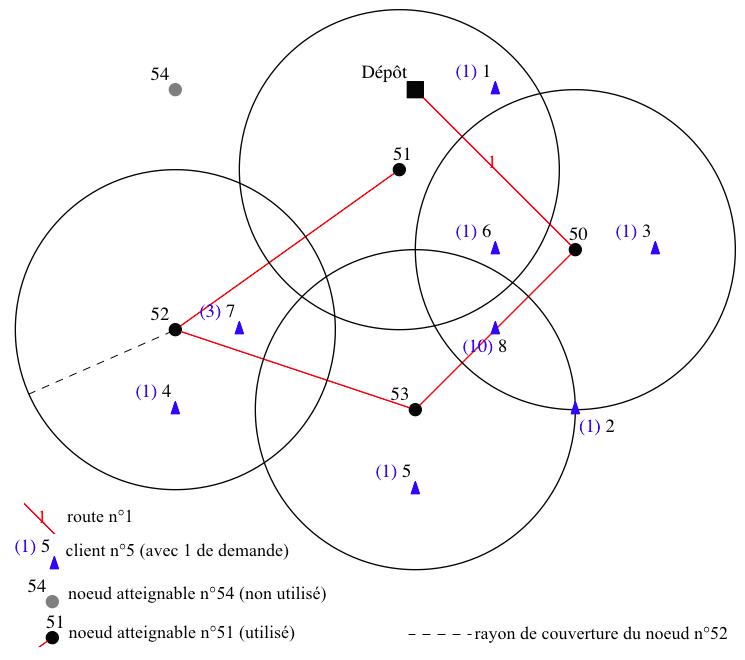
\includegraphics[width=0.999\textwidth]{figures/ctp_sans_vrp}
	\caption[Image générée par une corrélation]{Exemple de solution d'un CTP. Nous avons utilisé notre modèle de CTP-VRP en limitant le nombre de véhicules à un pour produire ce graphe.} \label{fig_correlation} 
\end{figure}


\begin{table}[h] \centering
\begin{tabular}{@{}llll@{}}
\toprule % utilise \usepackage{booktabs}
 & CTP avec VRP & CTP avec CCVRP & Écart relatif \\ \midrule
Nombre de camions & 2 & 2 & +0,0\% \\
Distance parcourue & 17,09 & 17,09 & +0,0\% \\
Somme des temps d'arrivée & 15,07 & 15,07 & +0,0\% \\
Temps d'arrivée maximal & 7,19 & 7,19 & +0,0\% \\ \bottomrule
\end{tabular}
\caption{Avec deux camions disponibles}
\label{deux_camions}
\end{table}

\begin{table}[h] \centering
\begin{tabular}{@{}llll@{}}
\toprule % utilise \usepackage{booktabs}
 & CTP avec VRP & CTP avec CCVRP & Écart relatif \\ \midrule
Nombre de camions & 2 & 3 & +50,0\% \\
Distance parcourue & 17,09 & 22,17 & +29,7\% \\
Somme des temps d'arrivée & 15,07 & 12,12 & -19,6\% \\
Temps d'arrivée maximal & 7,19 & 4,24 & -41,0\% \\ \bottomrule
\end{tabular}
\caption{Avec trois camions disponibles}
\label{trois_camions}
\end{table}

\begin{table}[h] \centering
\begin{tabular}{@{}llll@{}}
\toprule % utilise \usepackage{booktabs}
 & CTP avec VRP & CTP avec CCVRP & Écart relatif \\ \midrule
Nombre de camions & 2 & 4 & +100,0\% \\
Distance parcourue & 17,09 & 24,18 & +41,5\% \\
Somme des temps d'arrivée & 15,07 & 12,09 & -19,8\% \\
Temps d'arrivée maximal & 7,19 & 4,24 & -41,0\% \\ \bottomrule
\end{tabular}
\caption{Avec quatre camions disponibles}
\label{quatre_camions}
\end{table}

\section*{Annexes}
\subsection{Modèle mathématique du CTP-CCVRP}\label{modele}
\begin{equation}
Min \sum_{i=0}^{m}\sum_{j=0}^{m}\sum_{k=1}^{l}c_{ij}x_{ijk}
\end{equation}

s. t. :

\begin{equation}
\sum_{i=0}^{m}x_{ijk} = y_{jk}   j\in\left\{1,2,...,m\right\}, k\in\left\{1,2,...,l\right\}
\end{equation}

\begin{equation}
\sum_{i=0}^{m}x_{jik} = y_{jk}   j\in\left\{1,2,...,m\right\}, k\in\left\{1,2,...,l\right\}
\end{equation}

\begin{equation}
\sum_{j=0}^{m}x_{0jk} = 1   k\in\left\{1,2,...,l\right\}
\end{equation}

\begin{equation}
\sum_{j=0}^{m}x_{j0k} = 1   k\in\left\{1,2,...,l\right\}
\end{equation}

\begin{equation}
\sum_{j=1}^{m}\sum_{k=1}^{l}\alpha_{ij}D_{isjk} \geq d_{is}    i\in\left\{1,2,...,n\right\}, s\in\left\{1,2,...,t\right\}
\end{equation}

\begin{equation}
\sum_{i=1}^{n}\sum_{s=1}^{t}w{s}D_{isjk} \leq Q_{k}y_{jk}    k\in\left\{1,2,...,l\right\}, j\in\left\{1,2,...,m\right\}
\end{equation}

\begin{equation}
\sum_{s=1}^{t}\sum_{i=1}^{n}\sum_{j=1}^{m}w{s}D_{isjk} \leq Q_{k}    k\in\left\{1,2,...,l\right\}
\end{equation}

\begin{equation}
u_{ik} - u_{jk} + (m + 1)x_{ijk} \leq m   i,j\in\left\{1,2,...,m\right\}, k\in\left\{1,2,...,l\right\}
\end{equation}

\begin{equation}
x_{ijk} \in\left\{0,1\right\}   i,j\in\left\{1,2,...,m\right\}, k\in\left\{1,2,...,l\right\}
\end{equation}

\begin{equation}
y_{jk} \in\left\{0,1\right\}   j\in\left\{1,2,...,m\right\}, k\in\left\{1,2,...,l\right\}
\end{equation}

\begin{equation}
u_{ik} \geq 0   i\in\left\{1,2,...,m\right\}, k\in\left\{1,2,...,l\right\}
\end{equation}

\begin{equation}
D_{isjk} \geq 0   i\in\left\{1,2,...,n\right\}, s\in\left\{1,2,...,t\right\}, j\in\left\{1,2,...,m\right\}, k\in\left\{1,2,...,l\right\}
\end{equation}



\begin{equation}
u_{ik} - u_{jk} + Q_{k}x_{ijk} \leq Q_{k} - \sum_{s=1}^{t}\sum_{h=1}^{n}w_{s}D_{hsjk}   i,j\in\left\{1,2,...,m\right\}, k\in\left\{1,2,...,l\right\}
\end{equation}


\end{document}